\documentclass{article}
\usepackage{booktabs}
\usepackage{graphicx}
\usepackage{lipsum}
\usepackage{float}
\usepackage{subcaption}

\title{European Emergency Department Crowding Study}
\author{EEDCS consortium}

\begin{document}
\maketitle

\begin{abstract}
    \lipsum[1]    
\end{abstract}

\section{Introduction}
\lipsum[2]
\section{Materials and methods}
\lipsum[3]
\section{Results}


\subsection{Respondents}
\begin{table}[h]
\caption{Repondent positions}
\label{tab:respondents}
\begin{tabular}{lrrrrr}
\toprule
 & Head & Other & Resident & Specialist & Trainee \\
country &  &  &  &  &  \\
\midrule
Albania & 3 & 0 & 0 & 4 & 0 \\
Austria & 1 & 0 & 0 & 3 & 0 \\
Belgium & 1 & 0 & 0 & 0 & 0 \\
Croatia & 4 & 0 & 4 & 8 & 0 \\
Denmark & 1 & 0 & 3 & 10 & 0 \\
Estonia & 3 & 1 & 0 & 5 & 0 \\
Finland & 7 & 1 & 3 & 3 & 0 \\
France & 3 & 0 & 1 & 11 & 0 \\
Germany & 20 & 3 & 0 & 5 & 1 \\
Greece & 4 & 0 & 3 & 5 & 0 \\
Hungary & 7 & 0 & 1 & 3 & 0 \\
Iceland & 1 & 0 & 0 & 4 & 0 \\
Ireland & 1 & 0 & 1 & 5 & 1 \\
Italy & 8 & 3 & 0 & 9 & 0 \\
Lithuania & 0 & 0 & 0 & 1 & 0 \\
Malta & 0 & 0 & 0 & 7 & 1 \\
Netherlands & 0 & 0 & 0 & 6 & 0 \\
Norway & 3 & 0 & 0 & 1 & 0 \\
Poland & 8 & 1 & 3 & 4 & 0 \\
Romania & 3 & 0 & 0 & 2 & 0 \\
Slovenia & 2 & 0 & 1 & 1 & 0 \\
Spain & 3 & 1 & 0 & 9 & 0 \\
Sweden & 2 & 1 & 0 & 7 & 0 \\
Switzerland & 1 & 0 & 0 & 0 & 0 \\
Turkey & 0 & 6 & 16 & 14 & 3 \\
United Kingdom & 5 & 14 & 29 & 36 & 8 \\
\bottomrule
\end{tabular}
\end{table}


\begin{table}[h]
\caption{Hospital types}
\label{tab:hospitals}
\begin{tabular}{lrrrrr}
\toprule
 & other & primary & secondary & specialized & tertiary \\
country &  &  &  &  &  \\
\midrule
Albania & 0 & 1 & 3 & 0 & 3 \\
Austria & 0 & 0 & 0 & 0 & 4 \\
Belgium & 0 & 0 & 0 & 0 & 1 \\
Croatia & 0 & 2 & 1 & 0 & 13 \\
Denmark & 0 & 0 & 8 & 0 & 6 \\
Estonia & 0 & 2 & 2 & 0 & 5 \\
Finland & 0 & 0 & 8 & 0 & 6 \\
France & 0 & 3 & 1 & 1 & 10 \\
Germany & 0 & 0 & 8 & 0 & 21 \\
Greece & 0 & 0 & 2 & 0 & 10 \\
Hungary & 1 & 0 & 5 & 0 & 5 \\
Iceland & 0 & 1 & 0 & 0 & 4 \\
Ireland & 1 & 0 & 2 & 0 & 5 \\
Italy & 0 & 3 & 4 & 2 & 11 \\
Lithuania & 0 & 0 & 0 & 0 & 1 \\
Malta & 0 & 1 & 1 & 0 & 6 \\
Netherlands & 0 & 0 & 4 & 0 & 2 \\
Norway & 0 & 0 & 3 & 0 & 1 \\
Poland & 1 & 0 & 6 & 0 & 9 \\
Romania & 0 & 0 & 1 & 0 & 4 \\
Slovenia & 0 & 0 & 1 & 0 & 3 \\
Spain & 0 & 3 & 2 & 1 & 7 \\
Sweden & 1 & 2 & 2 & 0 & 5 \\
Switzerland & 0 & 0 & 0 & 0 & 1 \\
Turkey & 1 & 0 & 4 & 2 & 32 \\
United Kingdom & 2 & 5 & 49 & 3 & 33 \\
\bottomrule
\end{tabular}
\end{table}


\begin{figure}[H]
    \centering
        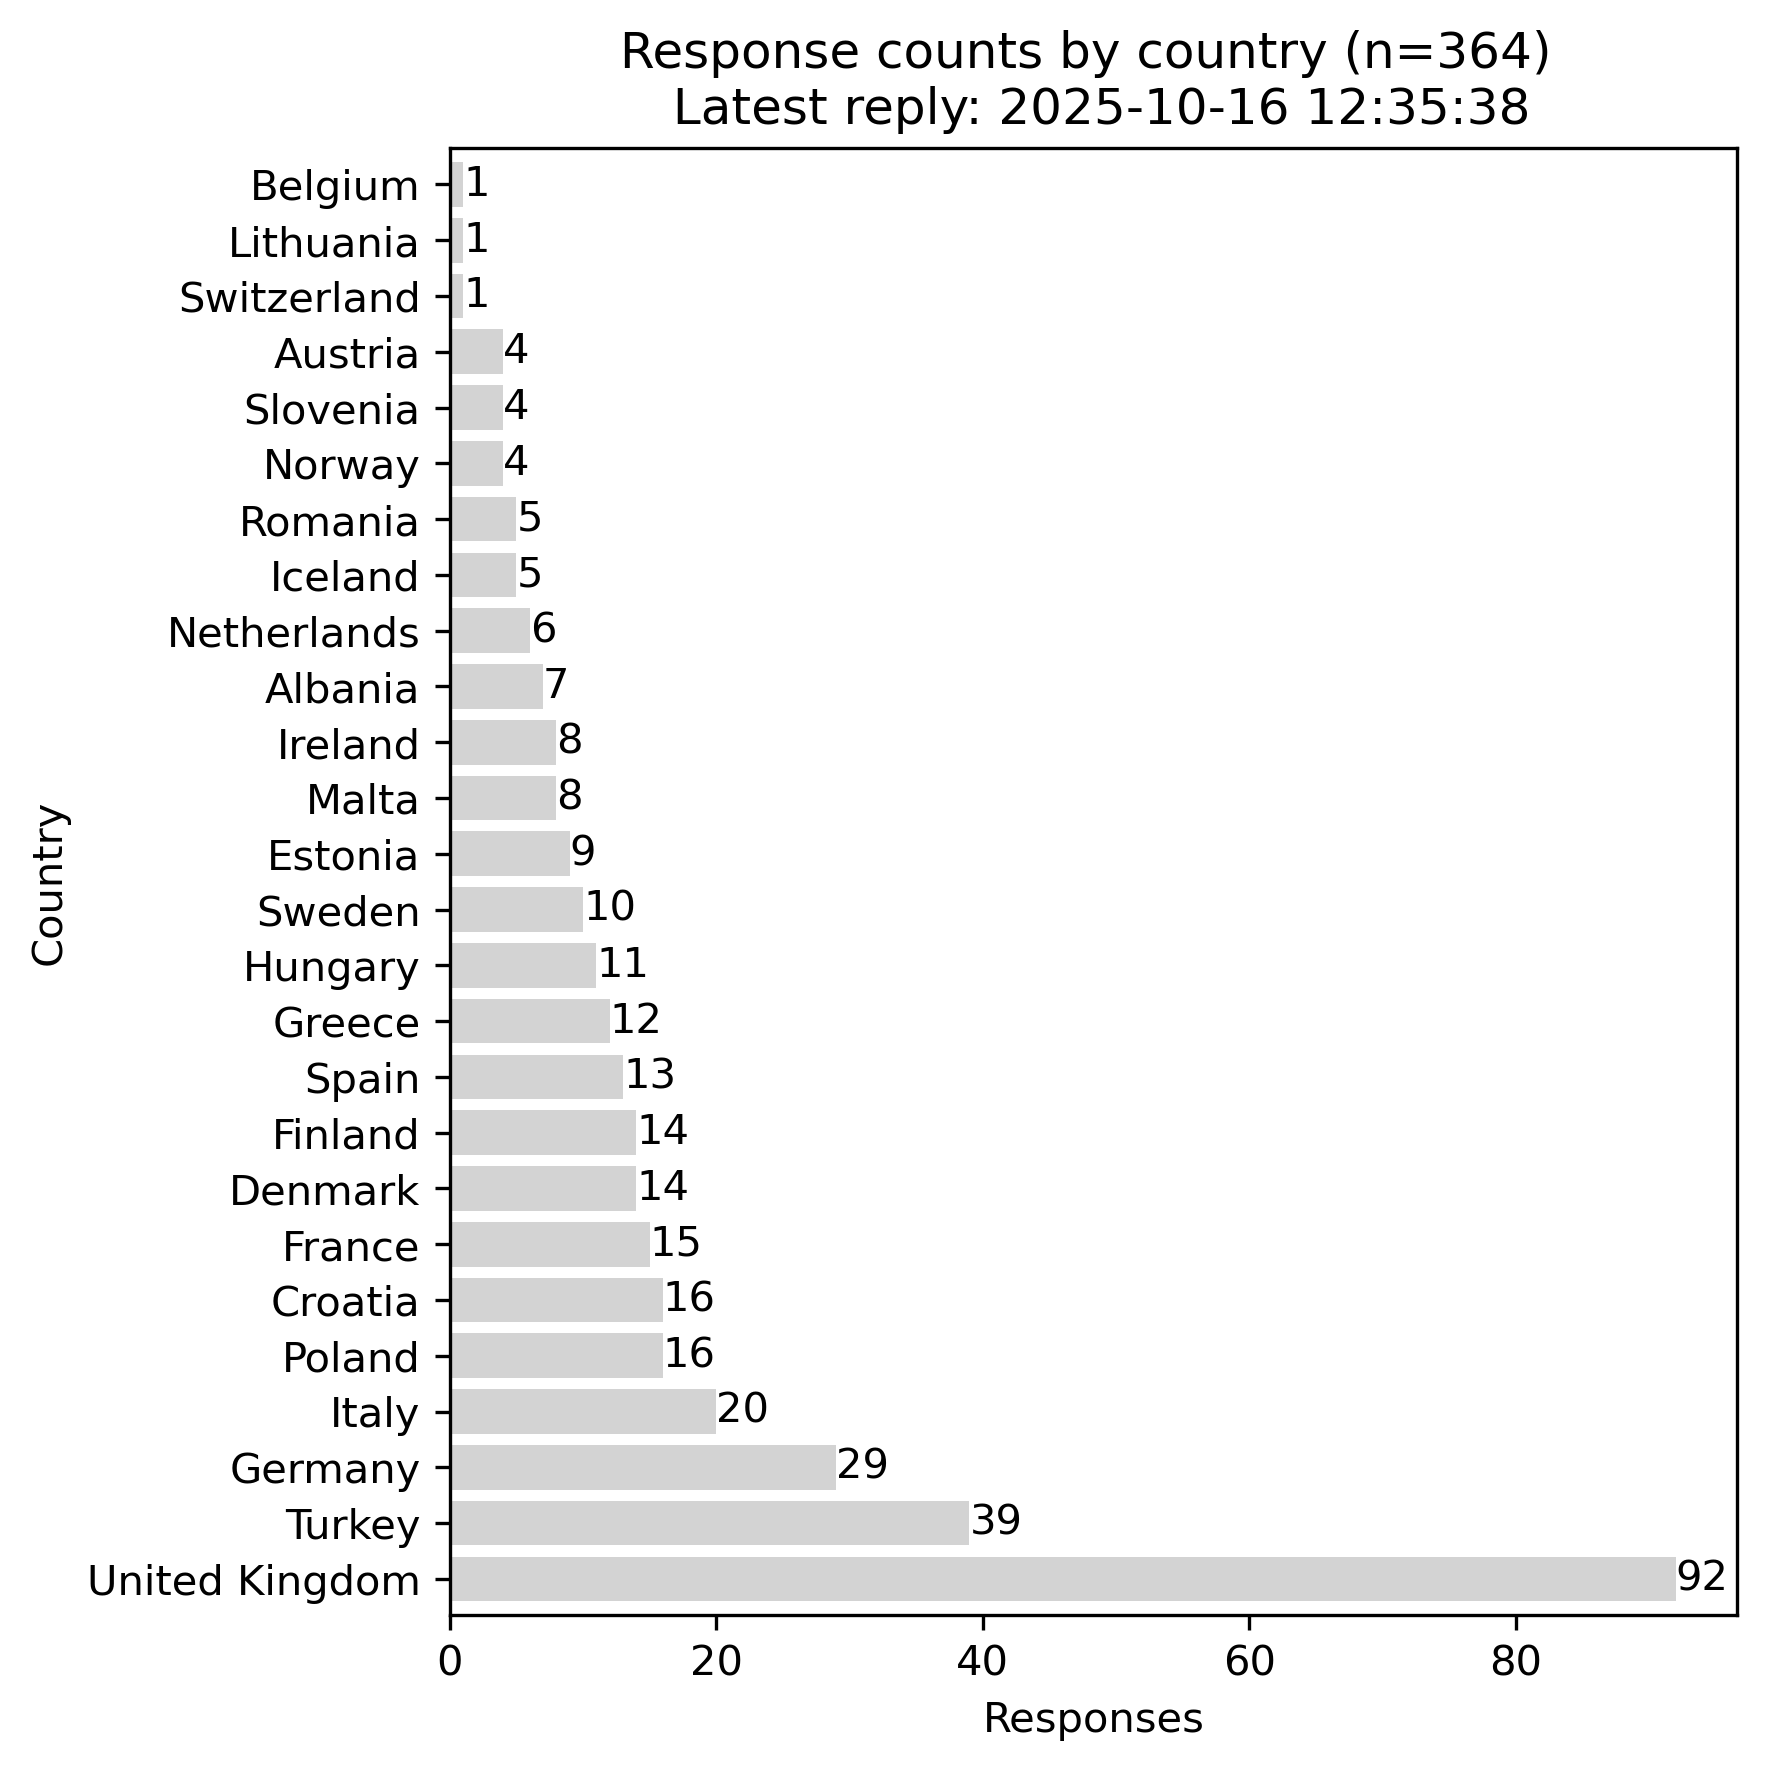
\includegraphics[width=0.7\textwidth]{../output/plots/country_freqs}
        \caption{countryfreqs}
        \label{fig:country_freqs}
\end{figure}

\subsection{Causes}

\lipsum[4]

\begin{figure}[p]
    \centering
        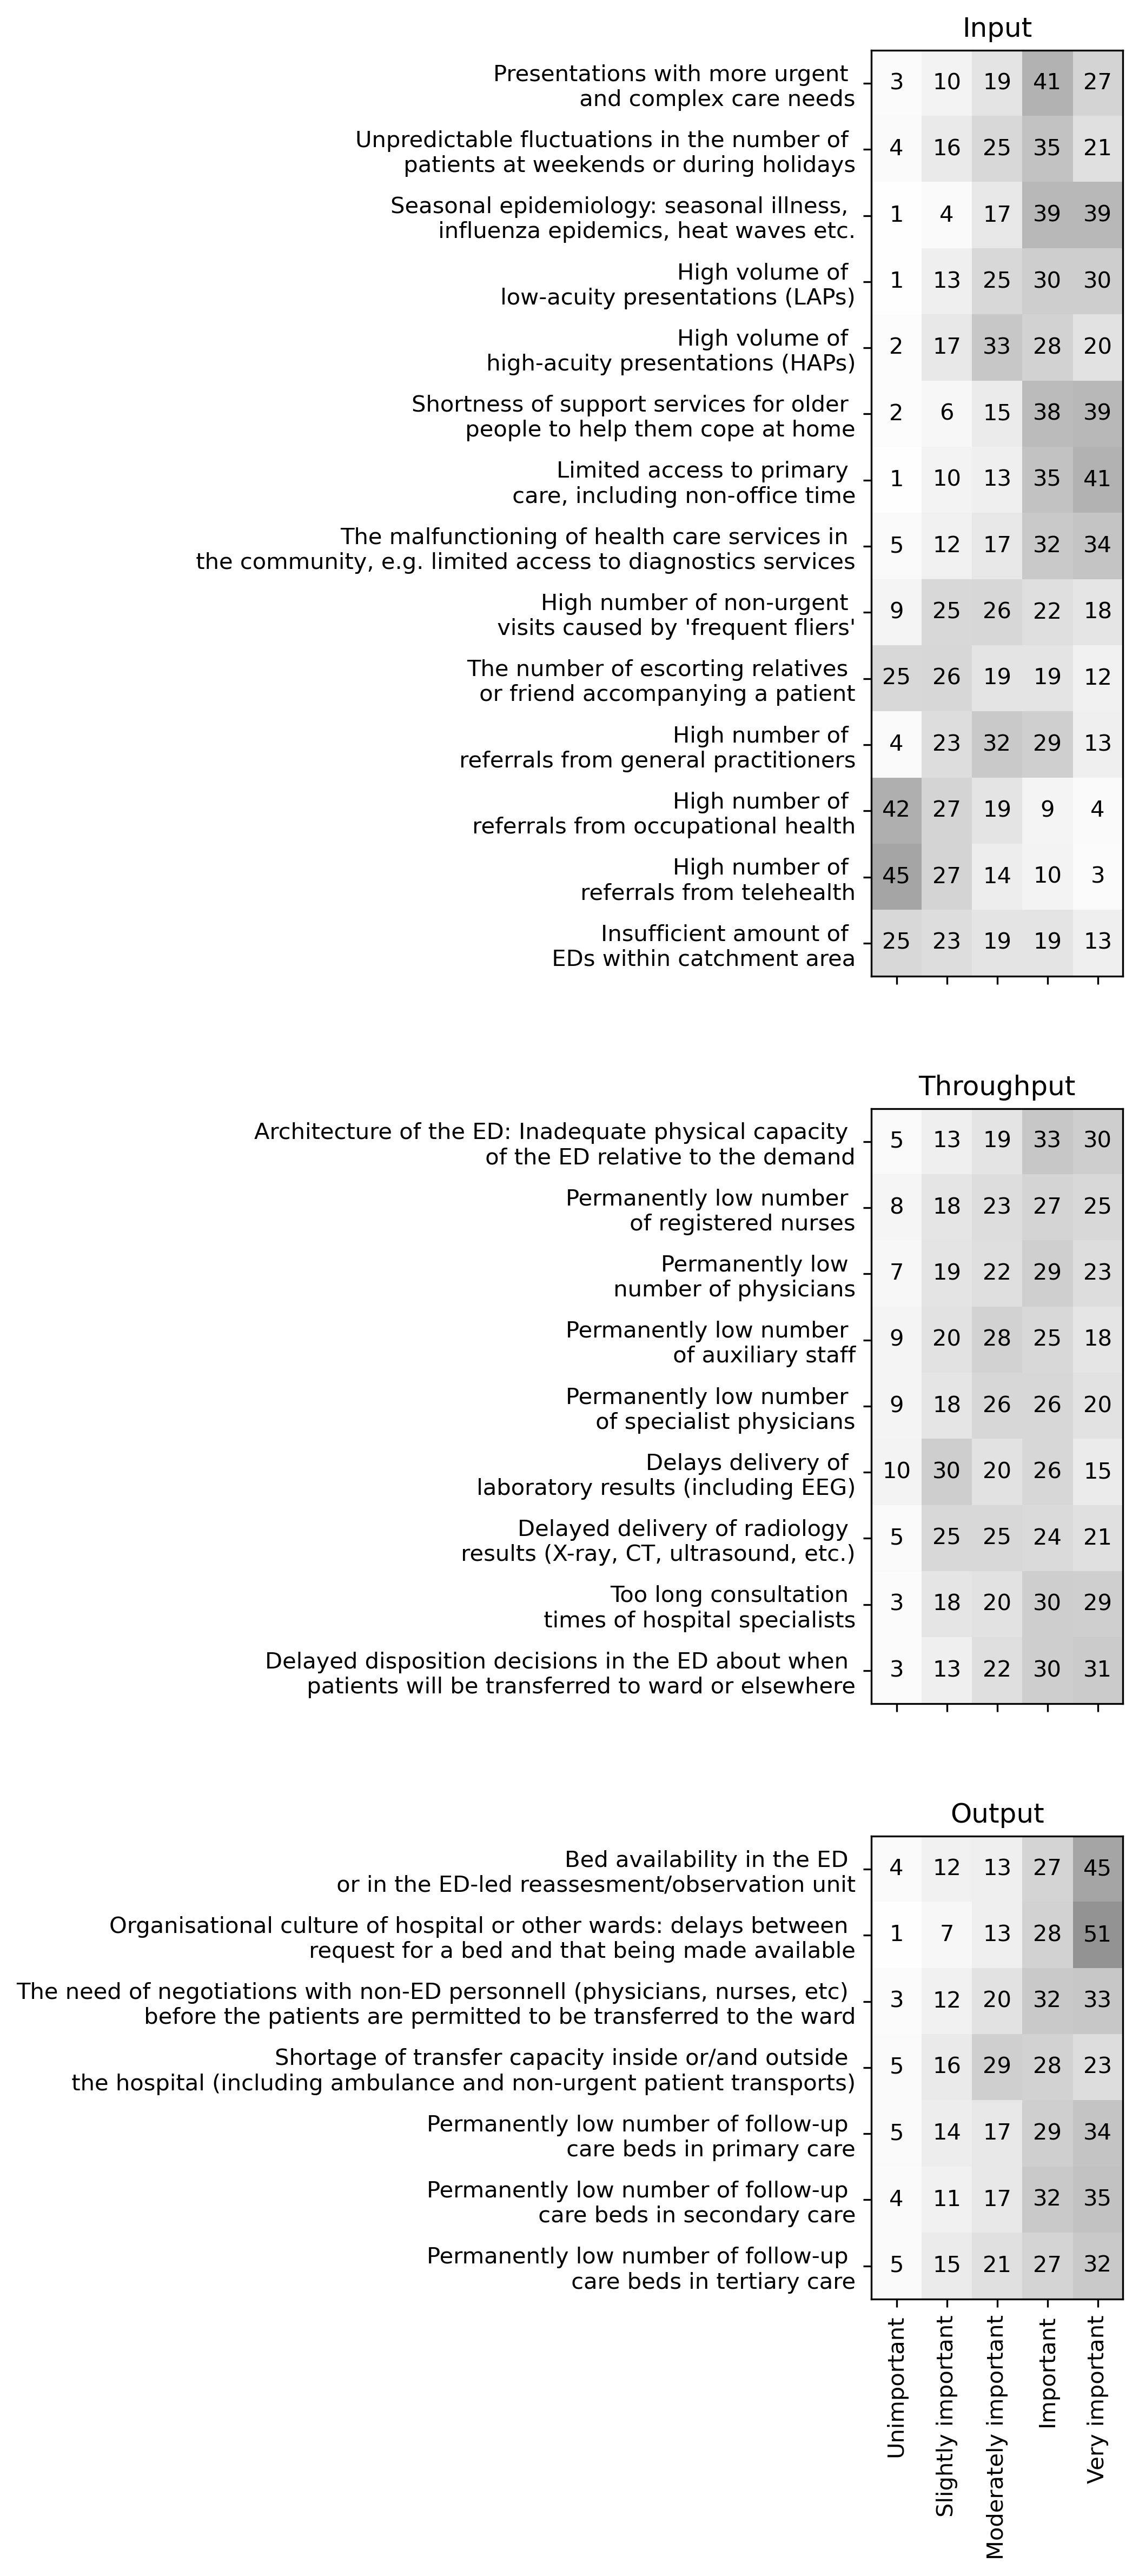
\includegraphics[height=1.0\textheight]{../output/plots/causes}
        \caption{causes}
        \label{fig:causes}
\end{figure}

\subsection{Operations management}

\begin{figure}[H]
    \centering
        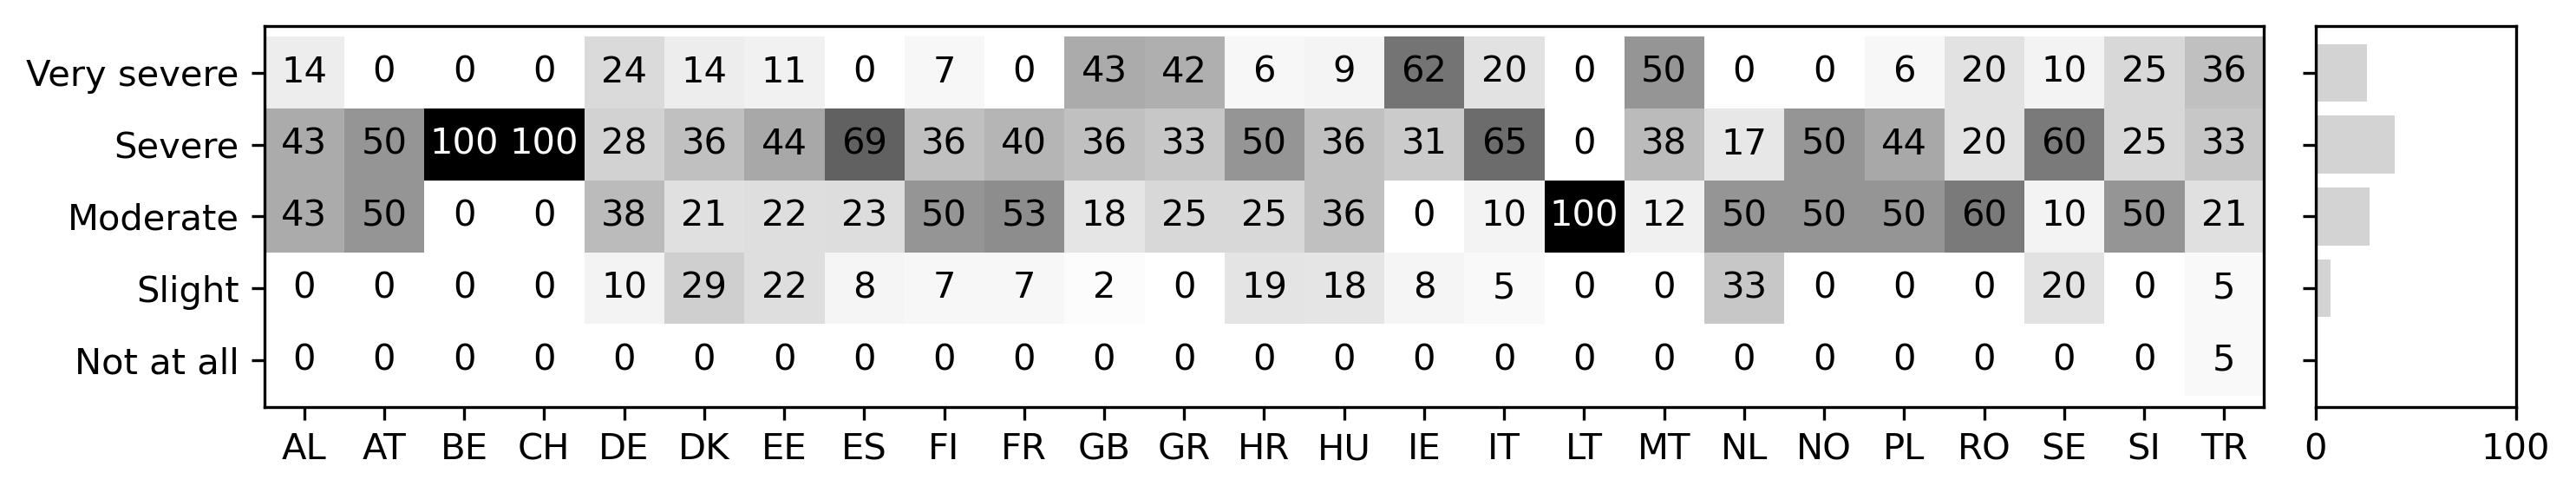
\includegraphics[width=0.5\textwidth]{../output/plots/severity}
        \caption{severity}
        \label{fig:severity}
\end{figure}

\begin{figure}[H]
    \centering
        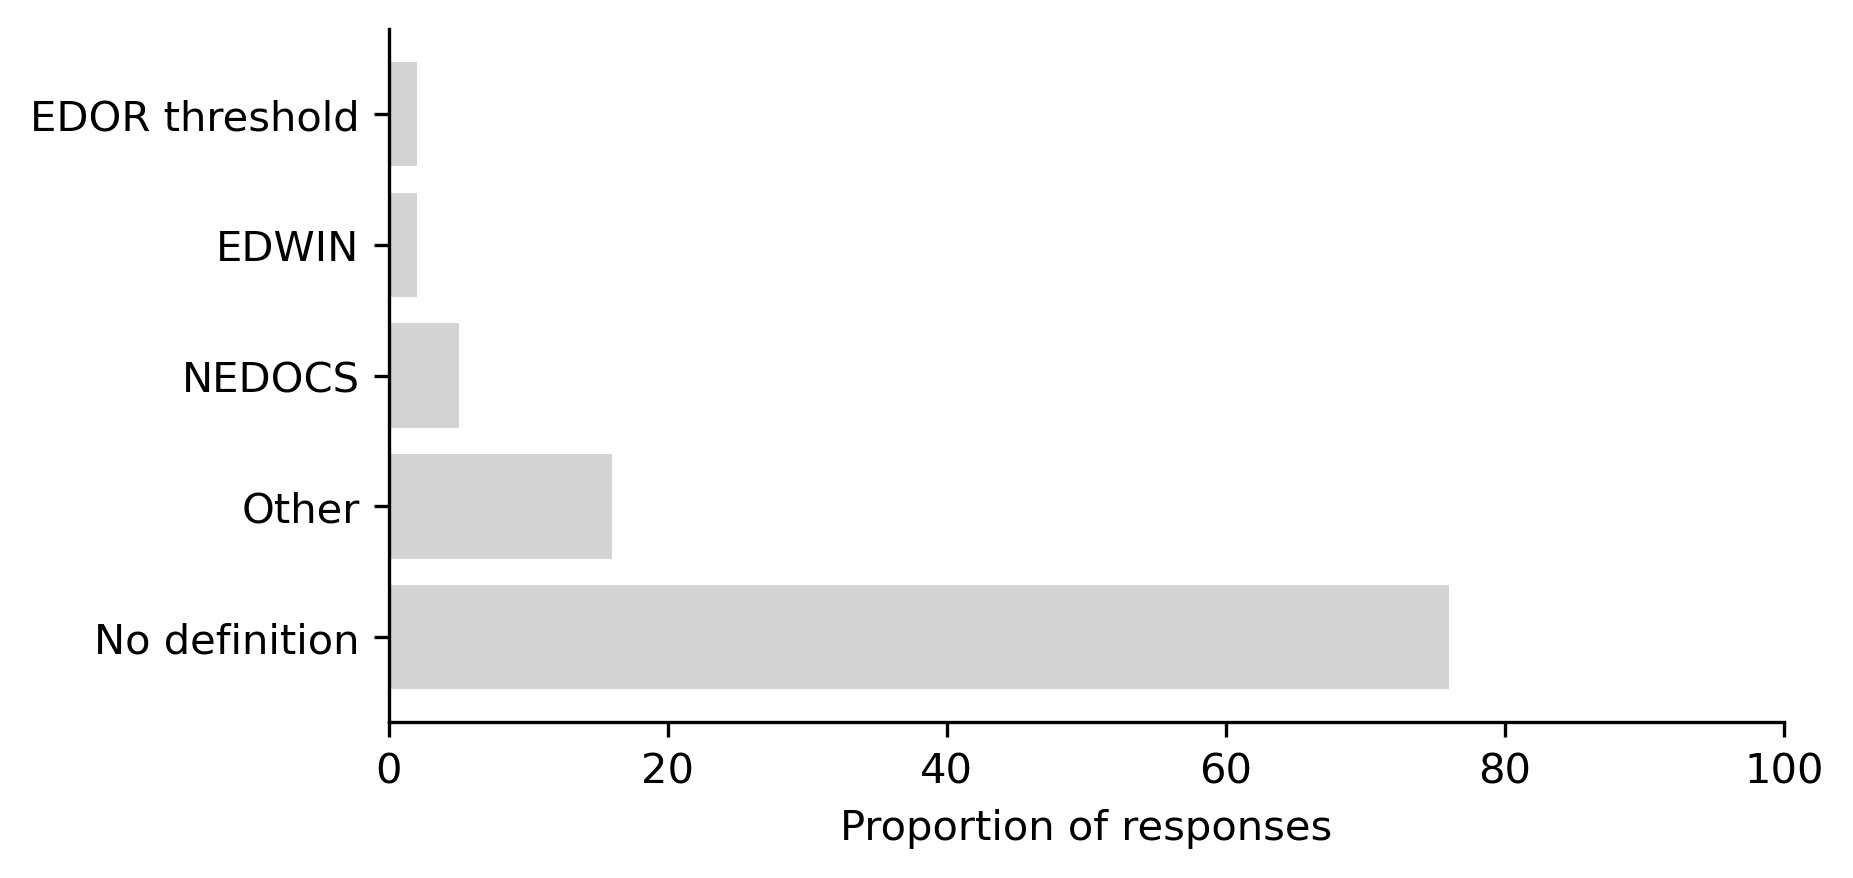
\includegraphics[width=1.0\textwidth]{../output/plots/definition}
        \caption{definition}
        \label{fig:definition}
\end{figure}

\begin{figure}[H]
    \centering
        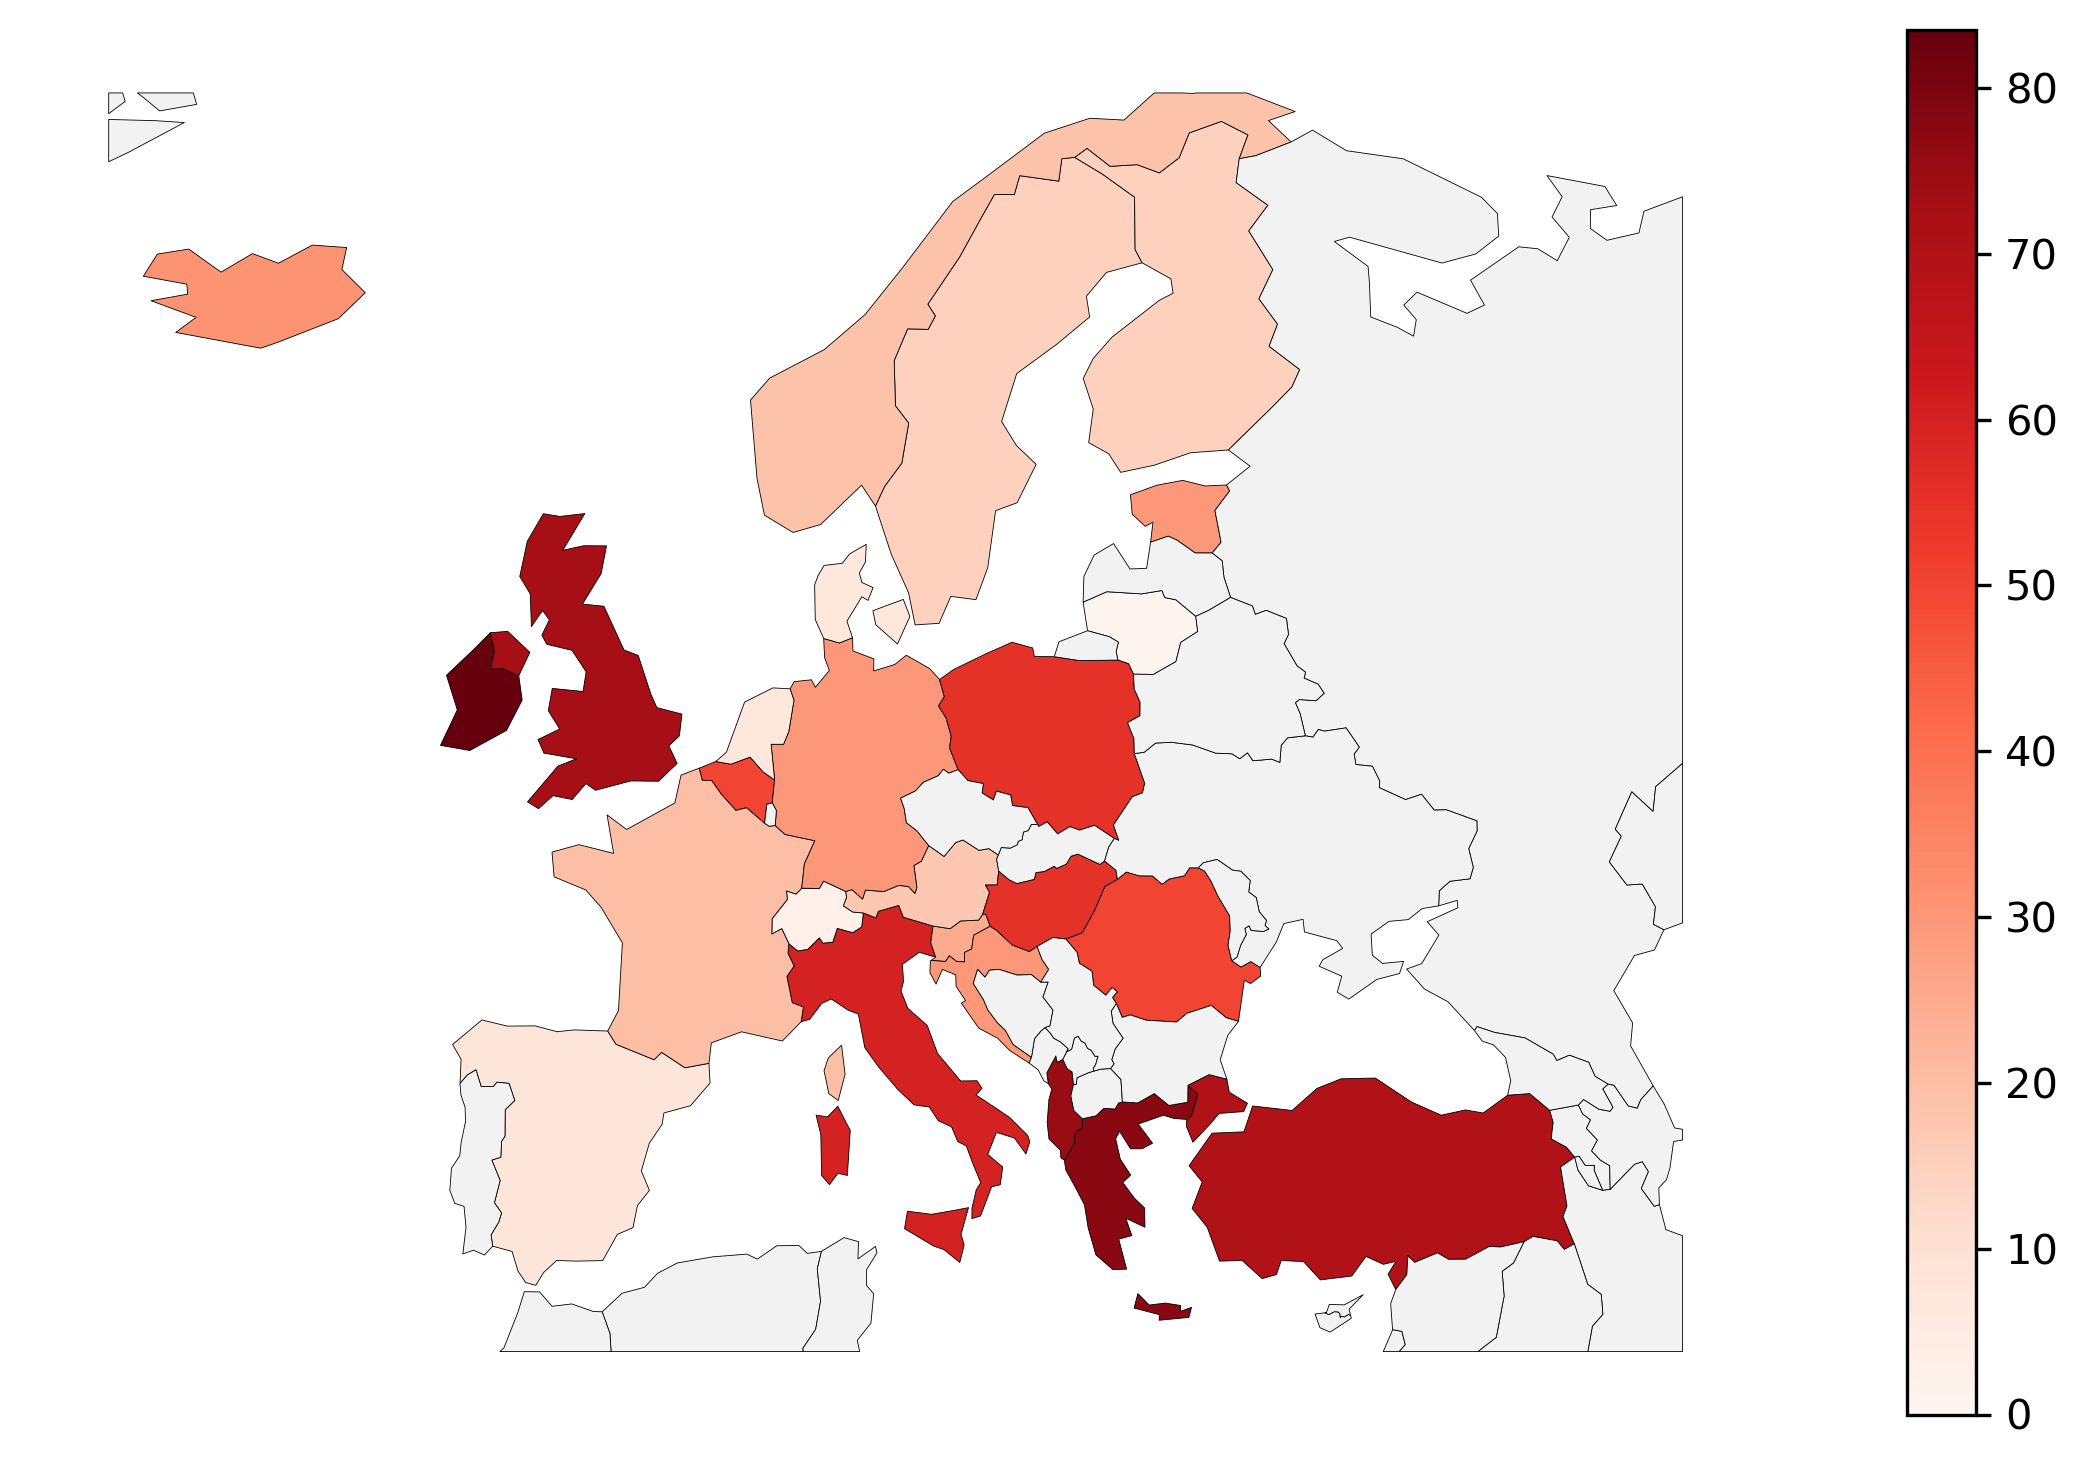
\includegraphics[width=1.0\textwidth]{../output/plots/crowding_map}
        \caption{Crowding map}
        \label{fig:crowding_map}
\end{figure}

\begin{figure}[H]
    \centering
        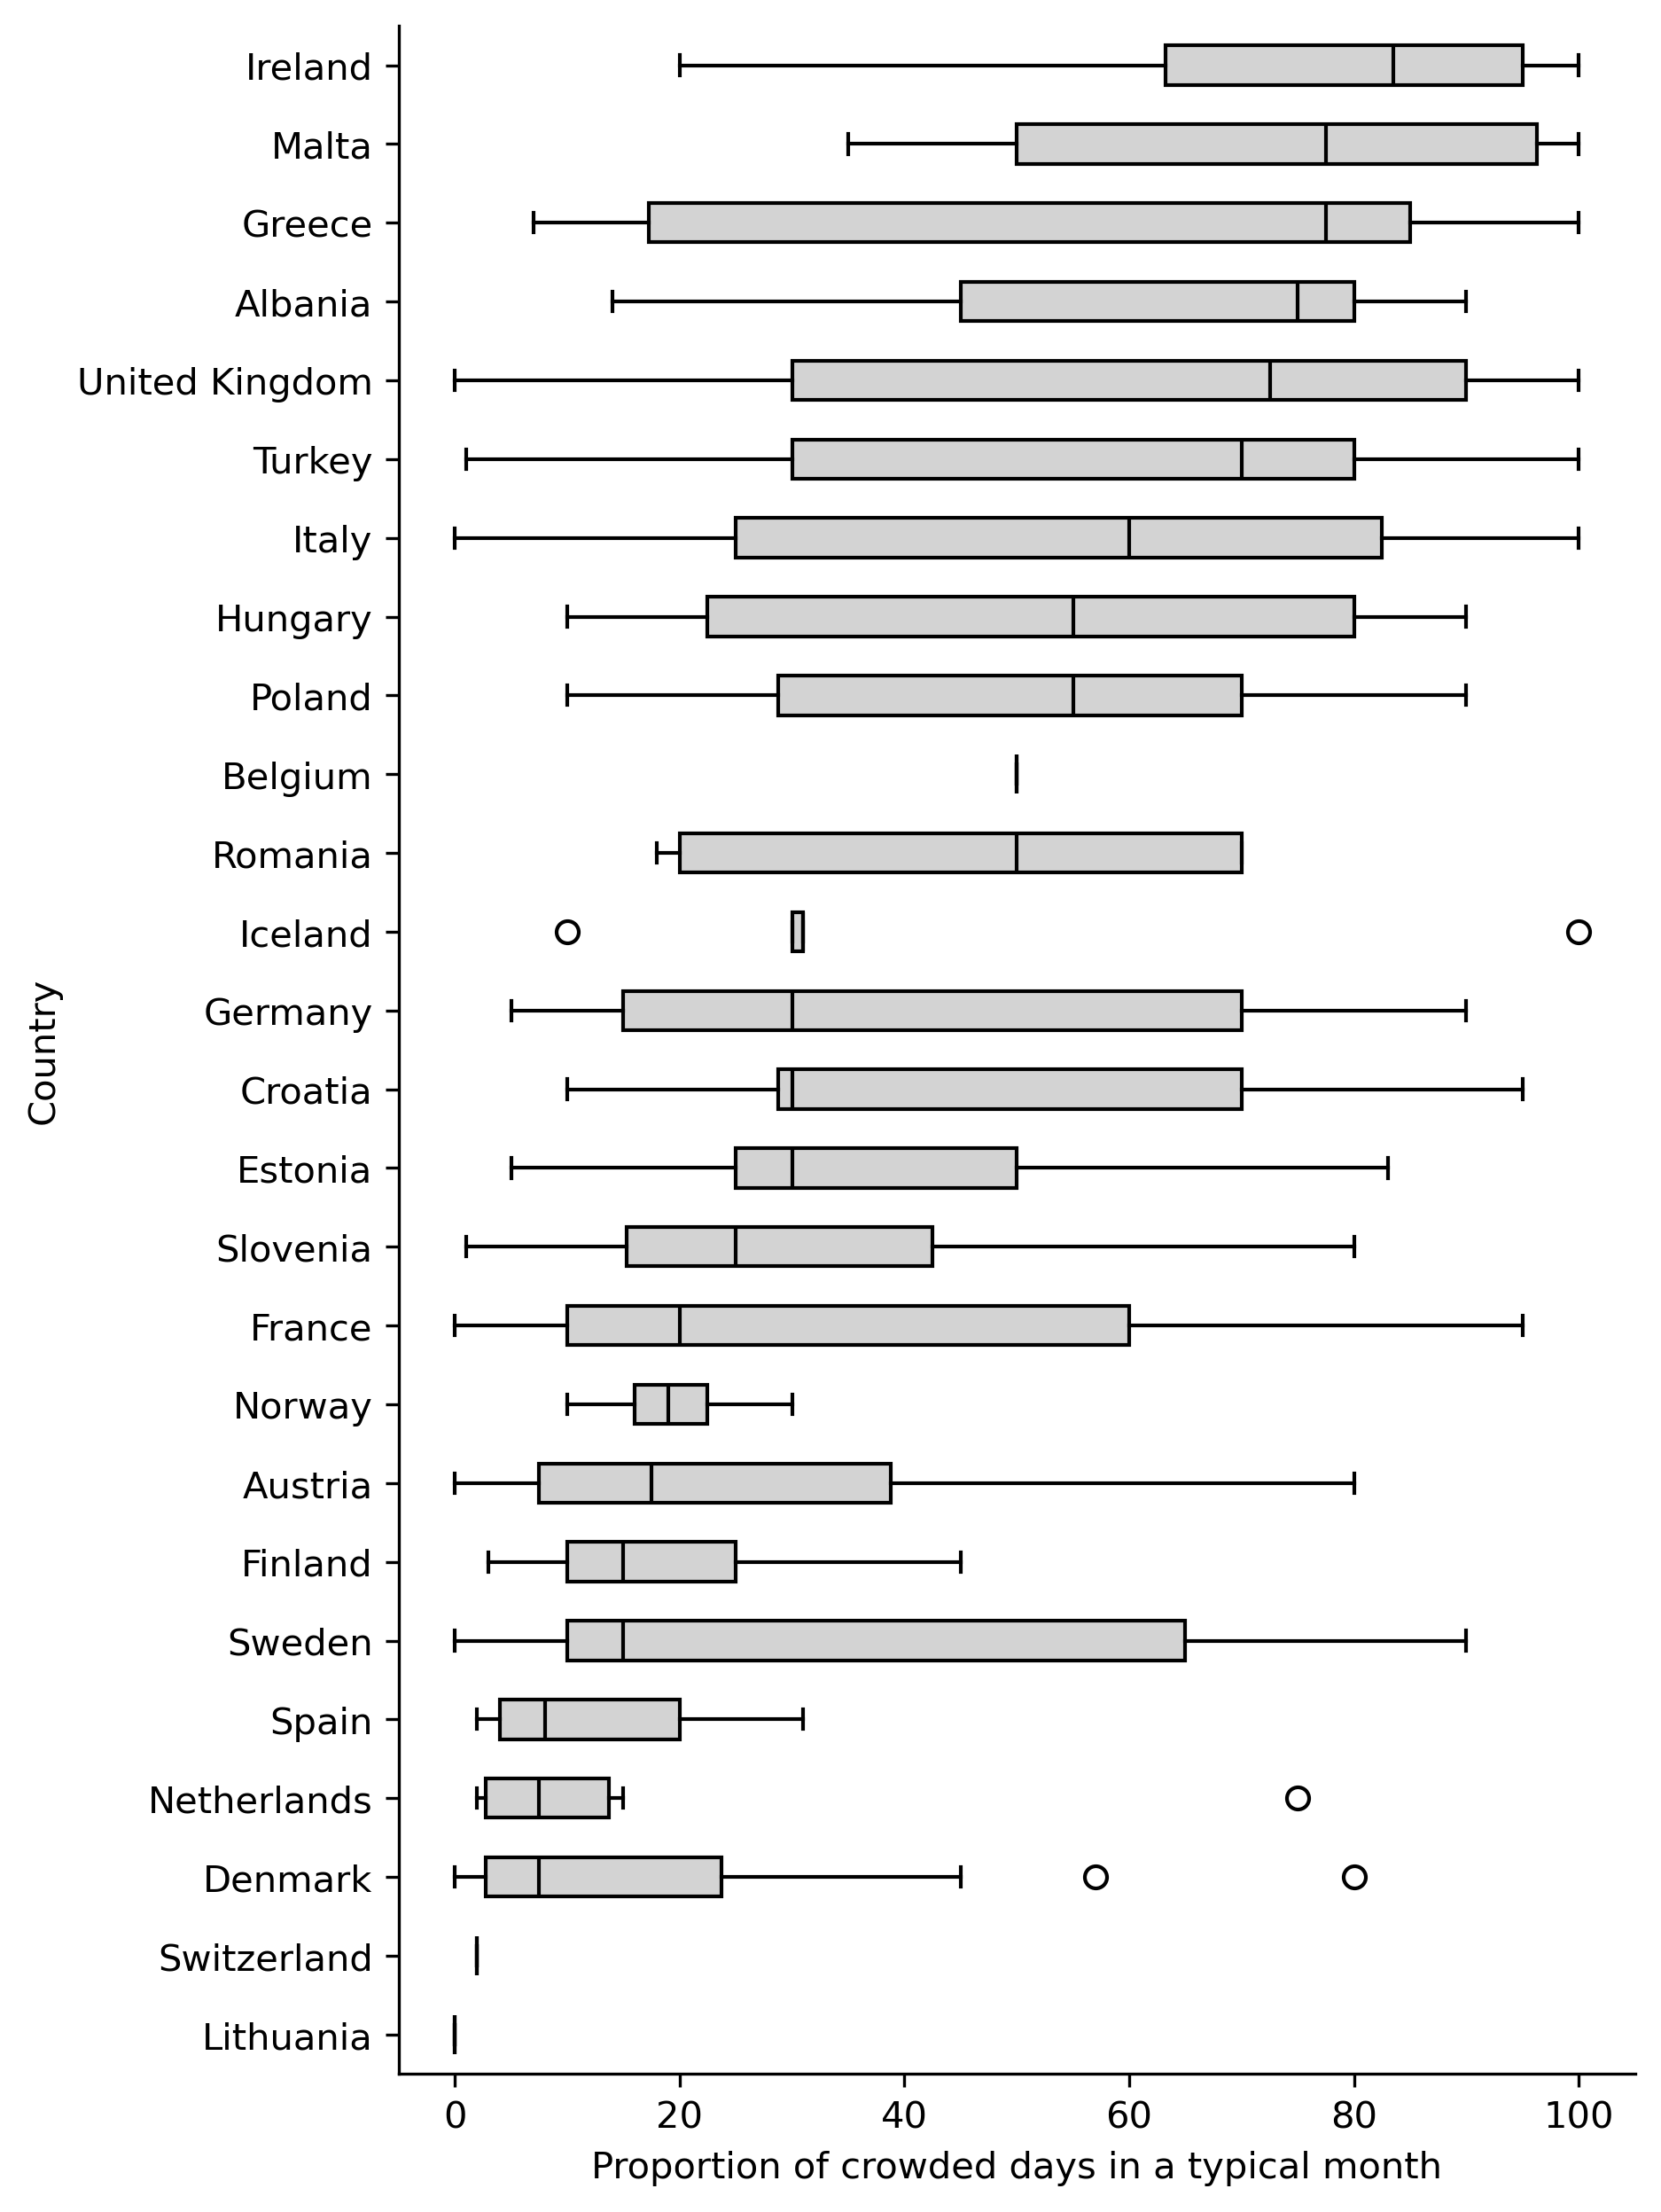
\includegraphics[width=0.7\textwidth]{../output/plots/country_crowding}
        \caption{countrycrowding}
        \label{fig:country_crowding}
\end{figure}

\begin{figure}[H]
    \centering
        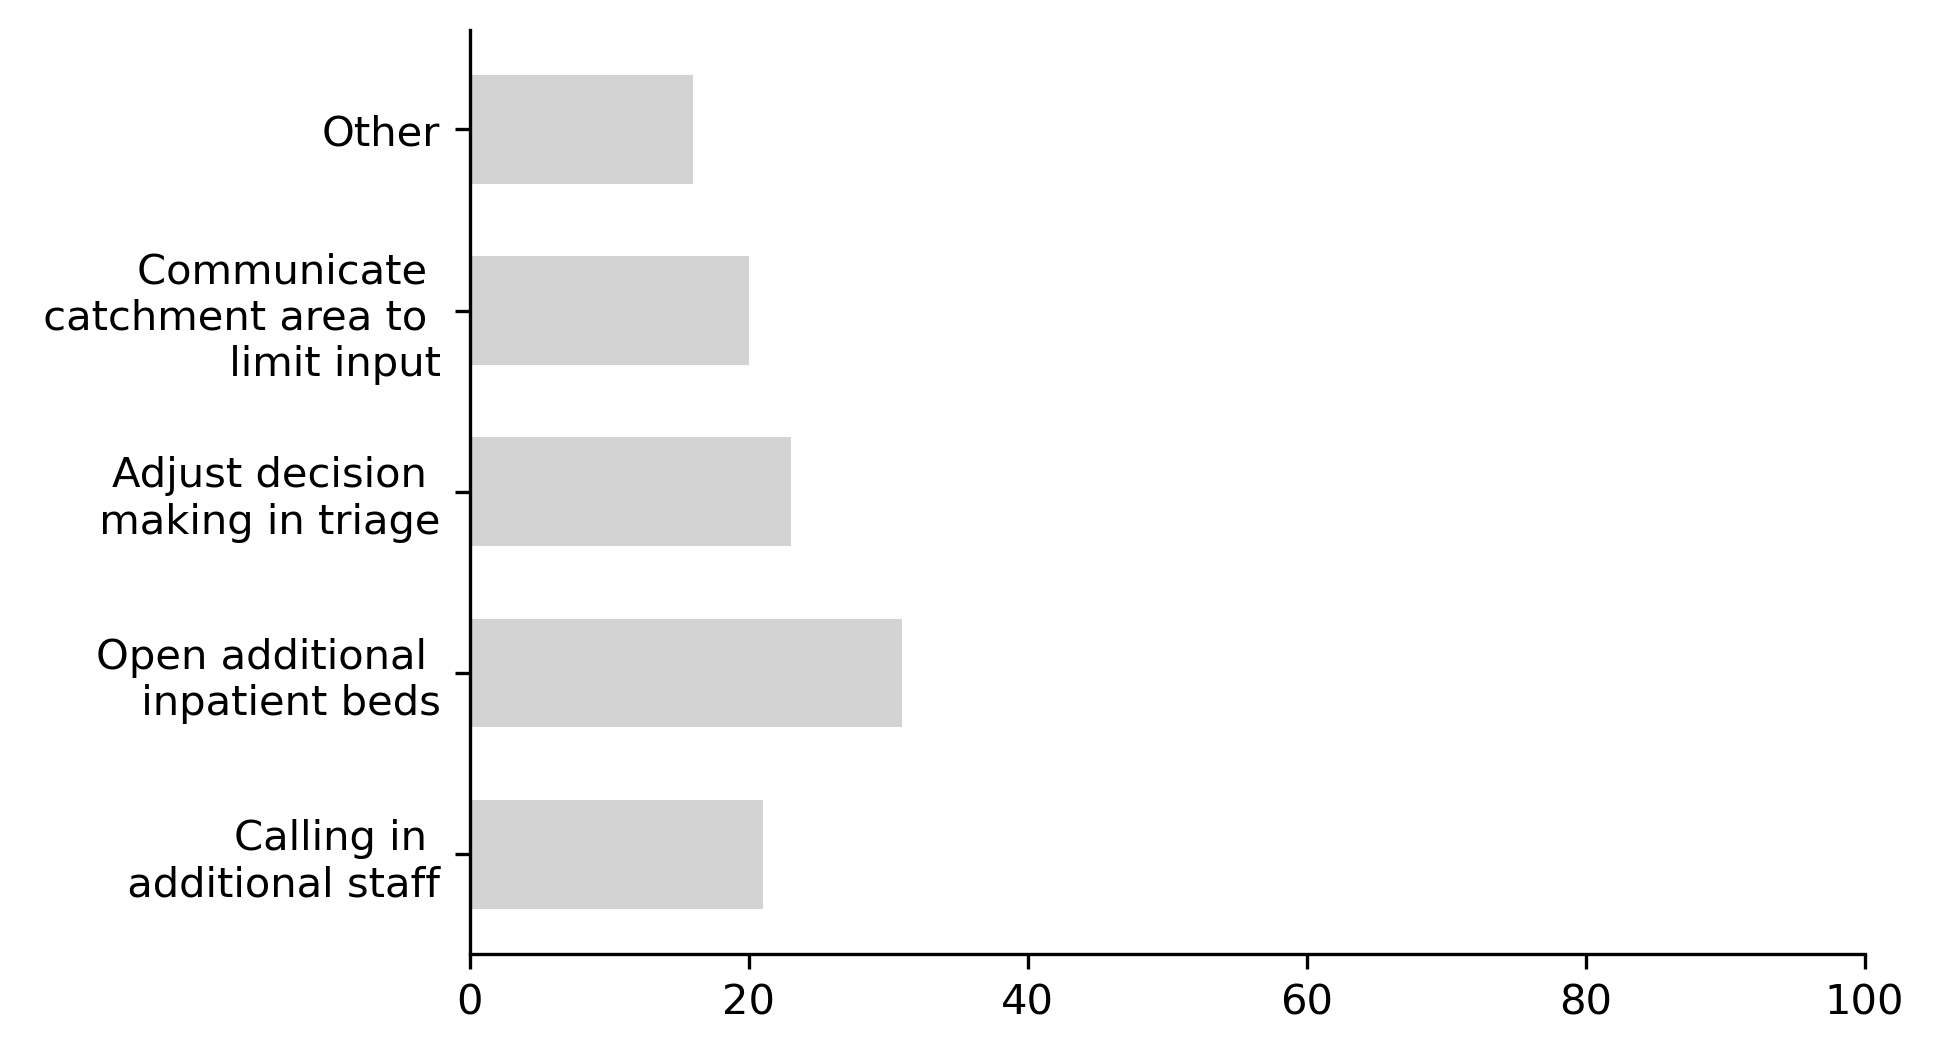
\includegraphics[width=1.0\textwidth]{../output/plots/interventions}
        \caption{Interventions}
        \label{fig:interventions}
\end{figure}

\subsection{Demand planning}

\begin{figure}[H]
    \centering
    \begin{subfigure}[b]{0.45\textwidth}
        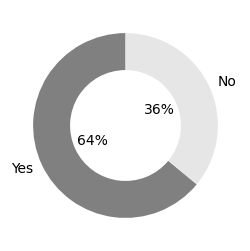
\includegraphics[width=\textwidth]{../output/plots/benefit}
        \caption{Would sufficiently accurate patient volume forecasting or crowding early warning software help alleviate the crowding problem?}
        \label{fig:benefit}
    \end{subfigure}
    \begin{subfigure}[b]{0.45\textwidth}
        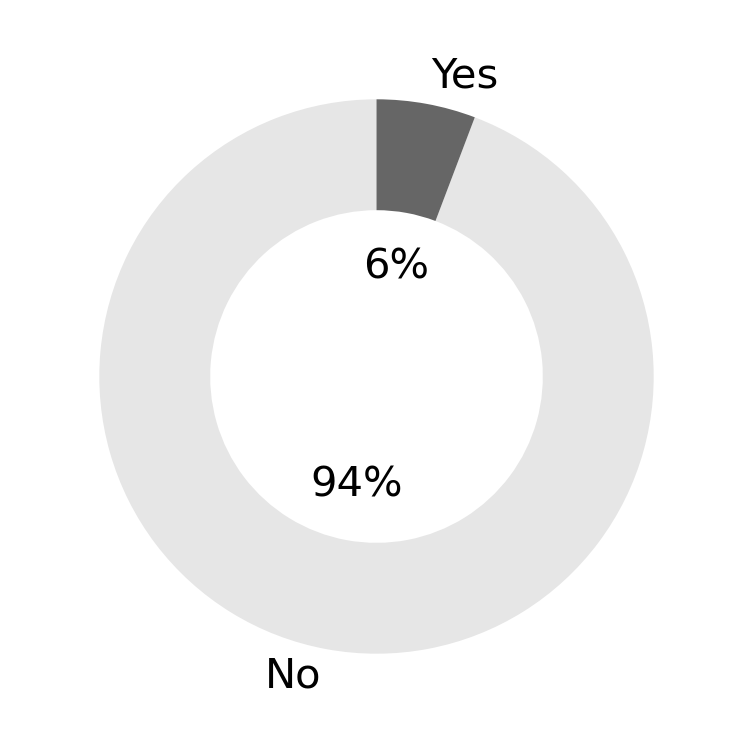
\includegraphics[width=\textwidth]{../output/plots/software_usage}
        \caption{Do you currently use a patient volume forecasting or crowding early warning software to guide decision making?}
        \label{fig:software_usage}
    \end{subfigure}
    \caption{}
    \label{fig:software_usage}
\end{figure}

\begin{figure}[H]
    \centering
        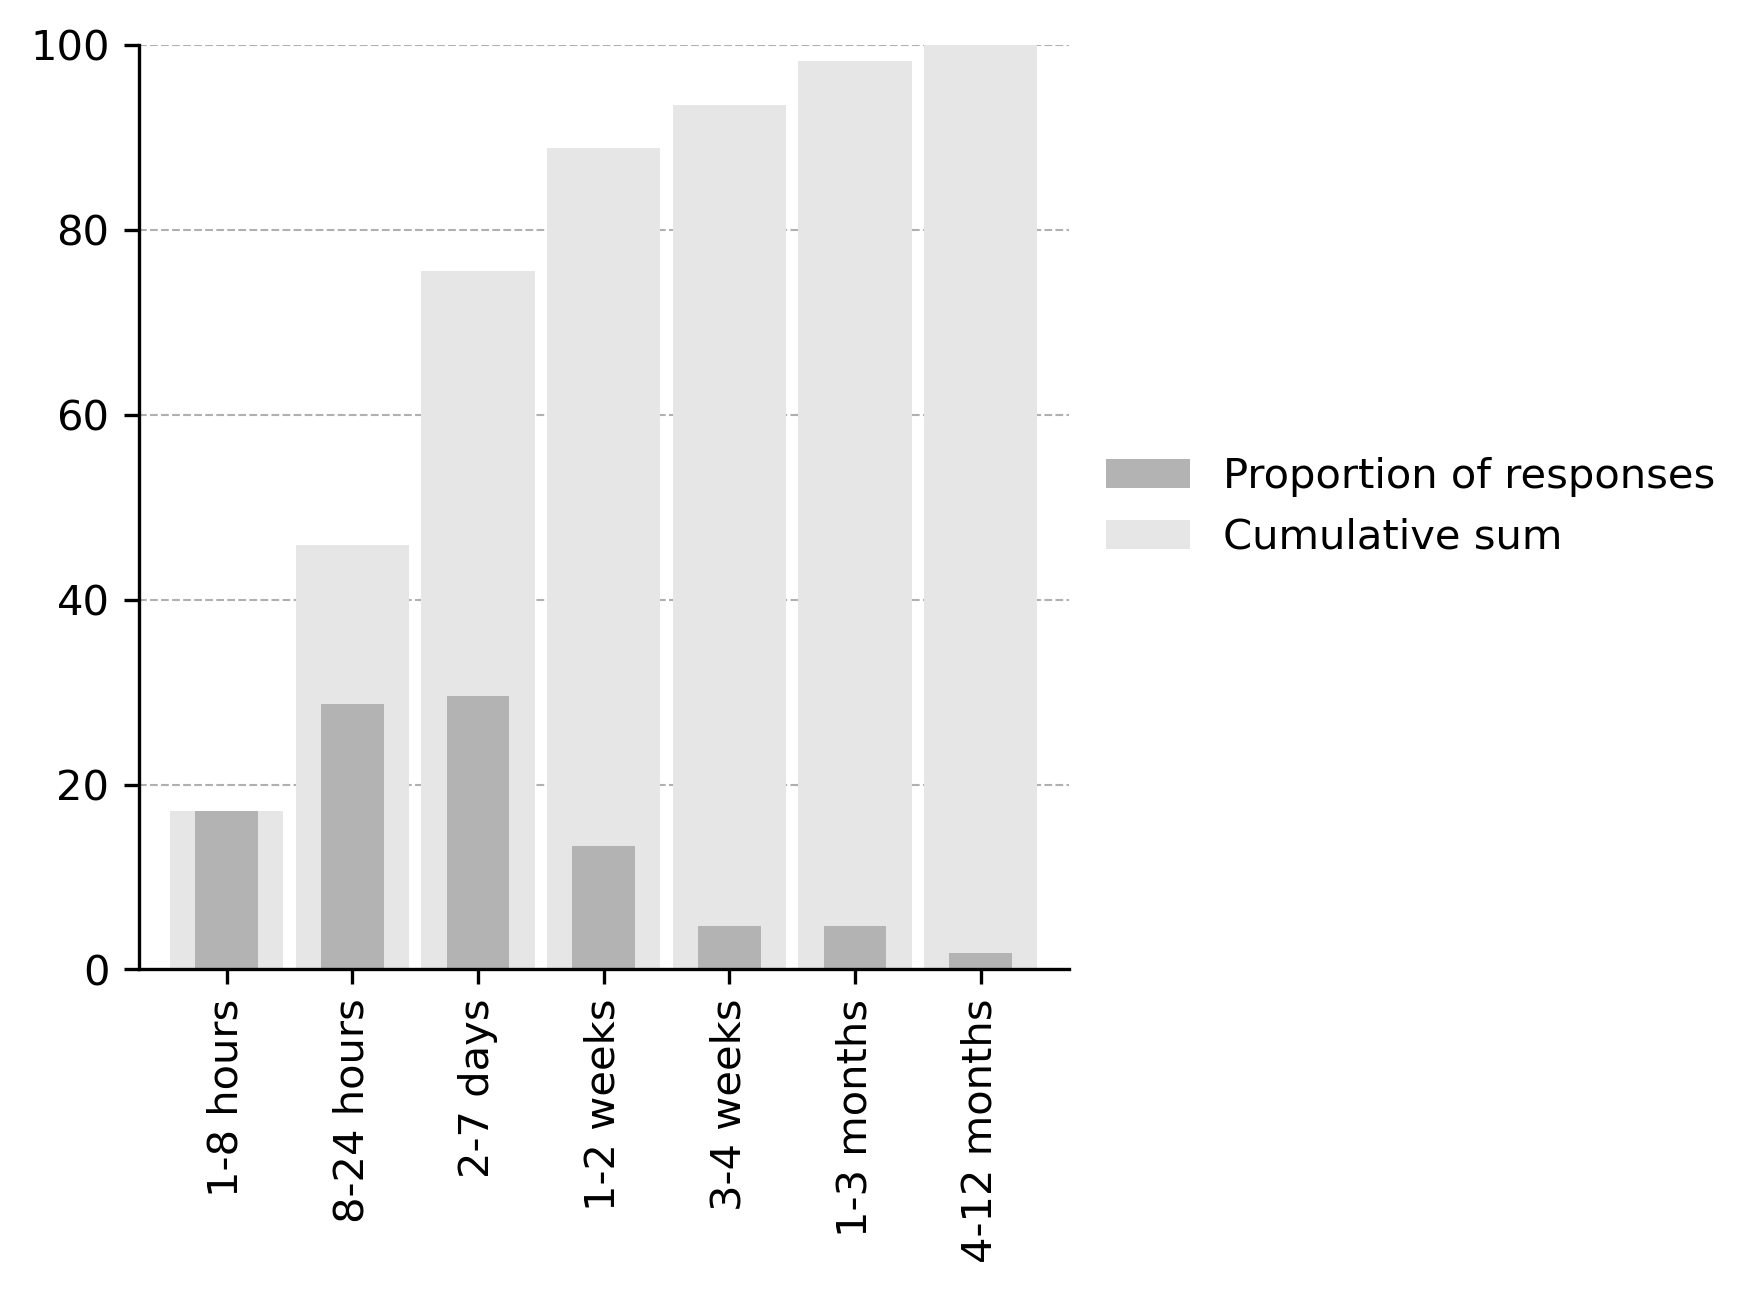
\includegraphics[width=1.0\textwidth]{../output/plots/horizon}
        \caption{Horizon}
        \label{fig:horizon}
\end{figure}

\section{Discussion}
\lipsum[5]

\end{document}